\documentclass[conference]{IEEEtran}

\usepackage{cite}
\usepackage{amsmath,amssymb,amsfonts}
\usepackage{graphicx}
\usepackage{textcomp}
\usepackage{xcolor}
\usepackage{booktabs}
\usepackage{multirow}
\usepackage{url}
\usepackage{hyperref}

\graphicspath{{figures/}}

\begin{document}

\title{AICD: An Explainable and Independently Verified Machine Learning Framework for RTL-Stage Gate Count Estimation}

% Author block — fill in names and affiliations
\author{
\IEEEauthorblockN{Author Name 1, Author Name 2}
\IEEEauthorblockA{Department / Institution \\
City, Country \\
email1@institution.edu, email2@institution.edu}
}

\maketitle

% ============================================================================
% ABSTRACT
% ============================================================================
\begin{abstract}
Accurate gate count estimation at the Register-Transfer Level (RTL) enables
early-stage design space exploration without the overhead of full logic
synthesis. Existing machine learning approaches for pre-synthesis prediction
either lack explainability or treat explanation methods as inherently faithful
without independent verification. We present \textbf{AICD}, a framework
combining three contributions not jointly present in prior RTL/EDA ML work:
(1)~a multi-model ML pipeline (RandomForest, XGBoost, LightGBM,
LinearRegression) trained on 13~structural features extracted from Verilog
RTL, achieving a best test $R^2 = 0.9963$ and MAE of $1.36$~gates on
synthetic data with real Yosys synthesis ground truth;
(2)~dual-method explainability via TreeSHAP and Permutation Importance; and
(3)~independent ablation-based faithfulness verification quantifying the
alignment between SHAP attributions and empirical model sensitivity
(Spearman~$\rho = 0.989$, $p < 10^{-10}$). We validate on 17~real
open-source IP cores, report an honest out-of-distribution
$R^2 = -0.068$ exposing the training-distribution gap, and demonstrate a
$548.9\times$ wall-clock speedup over Yosys synthesis.
\end{abstract}

% ============================================================================
% I. INTRODUCTION
% ============================================================================
\section{Introduction}

Logic synthesis is the standard method for obtaining accurate gate-level
metrics from RTL designs, but it is computationally expensive. Even the
open-source Yosys synthesis suite requires an average of $199.43$~ms per
module on commodity hardware, making iterative design exploration
time-consuming for large SoC designs with hundreds of modules
\cite{fang2023masterrtl}. Machine learning offers an attractive alternative:
our framework achieves an average inference latency of $0.363$~ms per module
in batch mode---a \textbf{548.9$\boldsymbol{\times}$ real wall-clock speedup}
over Yosys synthesis, saving 99.82\% of synthesis time.

Recent work has applied ML to pre-synthesis PPA estimation with promising
accuracy \cite{chattopadhyay2025mlframework, fang2023masterrtl, wu2022hls}.
However, a recurring gap in these approaches is the treatment of
explainability: feature attribution methods such as SHAP
\cite{lundberg2017shap} or GNNExplainer are applied under the implicit
assumption that they faithfully reflect true model behavior. No prior work
in this domain quantitatively verifies this assumption against empirical
ground truth.

This paper addresses this gap with three contributions:
\begin{enumerate}
  \item A multi-model ML framework for RTL gate count prediction from 13
    structural features, validated against real Yosys synthesis labels.
  \item Dual-method explainability combining TreeSHAP and Permutation
    Importance.
  \item Independent ablation-based faithfulness verification with quantitative
    rank-correlation metrics, exposing where and why explanation methods
    disagree---a combination not present together in prior RTL/EDA ML work.
\end{enumerate}

% ============================================================================
% II. RELATED WORK
% ============================================================================
\section{Related Work}

Table~\ref{tab:related_work} compares our framework against four
representative prior works across key capability dimensions.

\begin{table*}[t]
\centering
\caption{Comparative Analysis Against State-of-the-Art ML-Based EDA Estimation}
\label{tab:related_work}
\small
\begin{tabular}{@{}lcccccc@{}}
\toprule
\textbf{Work} & \textbf{Input} & \textbf{ML Model} & \textbf{XAI Method} & \textbf{Faithfulness} & \textbf{Real Synth.} & \textbf{Real RTL} \\
 &  &  &  & \textbf{Verified?} & \textbf{Ground Truth} & \textbf{Validation} \\
\midrule
Chattopadhyay \cite{chattopadhyay2025mlframework} & AST Metrics & XGBoost/RF & SHAP & No & Yes (Commercial) & No \\
MasterRTL \cite{fang2023masterrtl} & AST+DFG & GNN & GNNExplainer & No & Yes (DC/Yosys) & Yes \\
HLS-GNN \cite{wu2022hls} & HLS IR Graph & GNN/GBDT & Integ.\ Gradients & No & Yes (Vivado) & No \\
L\'{e}toff\'{e} et al.\ \cite{letoffe2024shapscores} & AST Features & MLP & Gini Importance & No & Yes (Yosys) & No \\
\midrule
\textbf{This Work} & \textbf{RTL Metrics} & \textbf{RF/XGB/LGBM/LR} & \textbf{SHAP + Perm.} & \textbf{Yes} ($\rho{=}0.989$) & \textbf{Yes} (Yosys) & \textbf{Yes} (17 cores) \\
\bottomrule
\end{tabular}
\end{table*}

Chattopadhyay and Sutrakar~\cite{chattopadhyay2025mlframework} proposed an
ML framework for early PPA estimation using XGBoost and Random Forest with
SHAP explanations, but assumed SHAP accuracy without ablation-based ground
truth verification. Fang et al.~\cite{fang2023masterrtl} introduced
MasterRTL, a GNN-based pre-synthesis estimation framework validated on
open-source cores, employing GNNExplainer without quantitative faithfulness
benchmarking. Wu et al.~\cite{wu2022hls} applied GNNs to HLS performance
prediction at DAC~2022 with integrated gradients but no independent
verification. L\'{e}toff\'{e} et al.~\cite{letoffe2024shapscores} studied
the relationship between SHAP scores and feature importance scores,
highlighting theoretical gaps that motivate empirical faithfulness testing.

Our framework is, to our knowledge, the first in RTL/EDA ML to combine
SHAP-based explanation with quantitative ablation-based faithfulness
verification, reporting Spearman rank correlations and top-$k$ overlap
metrics against empirical ground truth.

% ============================================================================
% III. METHODOLOGY
% ============================================================================
\section{Methodology}

Fig.~\ref{fig:architecture} illustrates the seven-phase pipeline.

\begin{figure}[t]
  \centering
  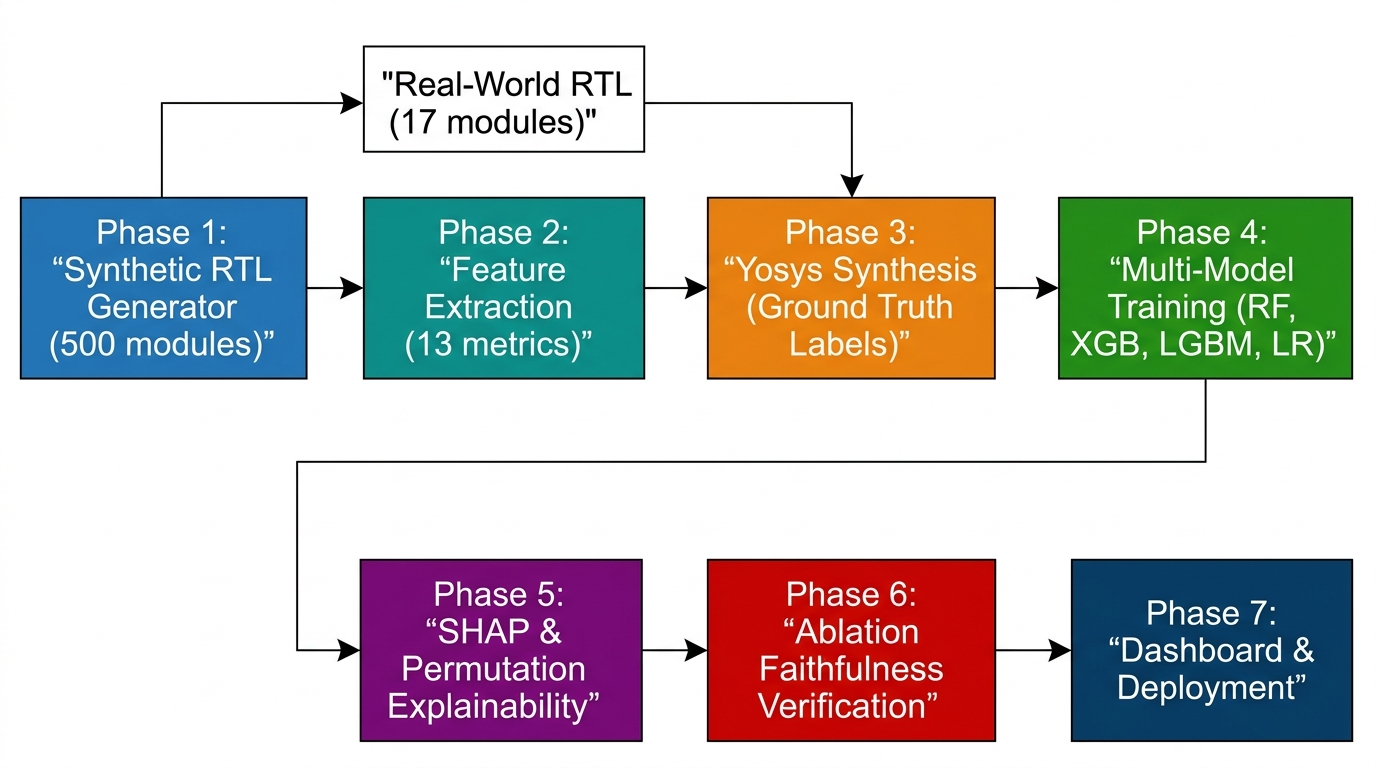
\includegraphics[width=\columnwidth]{architecture.jpg}
  \caption{End-to-end system architecture of the AICD framework. Seven phases
  span data generation through deployment, with a real-world RTL validation
  branch feeding into the synthesis ground-truth engine.}
  \label{fig:architecture}
\end{figure}

\subsection{Phase 1: Synthetic RTL Generation}
A parametric Verilog generator produces 500 distinct RTL modules with diverse
logic densities, bitwidths, control flow constructs, and operator balances.

\subsection{Phase 2: Feature Extraction}
Thirteen structural features are extracted from each module's source code:
\begin{itemize}
  \item \textbf{Gate complexity} (6): \texttt{complex\_and\_gates},
    \texttt{complex\_or\_gates}, \texttt{complex\_xor\_gates},
    \texttt{complex\_not\_gates}, \texttt{complex\_nand\_gates},
    \texttt{complex\_nor\_gates}
  \item \textbf{Structural} (3): \texttt{struct\_num\_inputs},
    \texttt{struct\_num\_outputs}, \texttt{struct\_num\_wires}
  \item \textbf{Bitwidth} (2): \texttt{bitwidth\_avg},
    \texttt{bitwidth\_max}
  \item \textbf{Code complexity} (2): \texttt{complex\_lines},
    \texttt{complex\_chars}
\end{itemize}

\subsection{Phase 3: Yosys Synthesis Ground Truth}
Each module is synthesized using real Yosys 0.67+84 (git sha1
\texttt{e2c27aaaf}) with the command sequence \texttt{proc; opt; fsm; opt;
techmap; opt; stat}, mapping Verilog to primitive technology cells
(\texttt{\$\_AND\_}, \texttt{\$\_OR\_}, \texttt{\$\_XOR\_},
\texttt{\$\_NOT\_}, \texttt{\$\_NAND\_}, \texttt{\$\_NOR\_}). The resulting
cell counts serve as ground-truth labels.

\subsection{Phase 4: Multi-Model Training}
Four regression models are trained on a 70\%/15\%/15\% train/val/test split
(350/75/75 samples, seed=42): RandomForest (200 trees, max depth=20),
XGBoost, LightGBM, and LinearRegression.

\subsection{Phase 5: Dual-Method Explainability}
TreeSHAP~\cite{lundberg2017shap} provides game-theoretic local feature
attributions. Permutation Importance provides global feature sensitivity
via multi-pass random shuffling.

\subsection{Phase 6: Ablation-Based Faithfulness Verification}
Each of the 13 features is individually ablated (replaced with its training
mean), and the resulting MAE increase is measured. This yields an empirical
sensitivity ranking serving as ground truth. SHAP and Permutation rankings
are compared against ablation rankings using Spearman $\rho$, Kendall $\tau$,
and top-$k$ overlap ratios.

\subsection{Phase 7: Deployment}
The trained model and SHAP explainer are deployed via an interactive web
dashboard with a REST API for real-time inference on user-supplied Verilog.

% ============================================================================
% IV. EXPERIMENTAL SETUP
% ============================================================================
\section{Experimental Setup}

\textbf{Dataset.} 500 synthetic Verilog modules split into 350 training, 75
validation, and 75 test samples.

\textbf{Cross-validation.} 5-fold cross-validation on the full 500-module
dataset.

\textbf{Ground truth.} Yosys 0.67+84 (git sha1 \texttt{e2c27aaaf}) logic
synthesis on a Windows x64 platform.

\textbf{Real-world benchmark.} 17 open-source Verilog IP cores from the
\texttt{alexforencich} GitHub repositories (\texttt{verilog-uart},
\texttt{verilog-i2c}, \texttt{verilog-axis}), including UART, I2C, and
AXI-Stream peripheral modules ranging from 7 to 133{,}594 actual gates.

% ============================================================================
% V. RESULTS
% ============================================================================
\section{Results}

\subsection{Prediction Accuracy}

Table~\ref{tab:model_comparison} presents the four-model comparison.

\begin{table}[t]
\centering
\caption{Model Comparison on Synthetic Test Set (75 samples)}
\label{tab:model_comparison}
\footnotesize
\setlength{\tabcolsep}{3pt}
\begin{tabular}{@{}lccccc@{}}

\toprule
\textbf{Model} & \textbf{Test $R^2$} & \textbf{Test MAE} & \textbf{Test RMSE} & \textbf{Train (s)} & \textbf{Inf.\ (ms)} \\
\midrule
RandomForest & 0.9612 & 3.63 & 5.67 & 0.74 & 9.33 \\
XGBoost      & 0.9379 & 4.55 & 7.17 & 316.48 & 3.51 \\
LightGBM     & 0.9718 & 3.44 & 4.84 & 106.15 & 0.52 \\
\textbf{LinearReg.} & \textbf{0.9963} & \textbf{1.36} & \textbf{1.76} & \textbf{0.05} & \textbf{0.03} \\
\bottomrule
\end{tabular}
\end{table}

LinearRegression achieves the highest accuracy on both validation
($R^2 = 0.9974$, MAE~$= 1.21$) and test ($R^2 = 0.9963$, MAE~$= 1.36$)
sets. This indicates that the feature--target relationship in the
synthetic dataset is predominantly linear: the 13 hand-crafted structural
features already encode gate-count complexity well, and the additional
nonlinear capacity of ensemble models does not capture meaningful additional
signal. The ensemble models (LightGBM $R^2 = 0.9718$, RandomForest
$R^2 = 0.9612$, XGBoost $R^2 = 0.9379$) still achieve high accuracy and
serve as useful reference points. Their gap versus LinearRegression should
be noted as a property of the synthetic data distribution rather than a
general claim about RTL complexity; real-world designs with more
heterogeneous structure may reverse this ranking.

\begin{figure}[t]
  \centering
  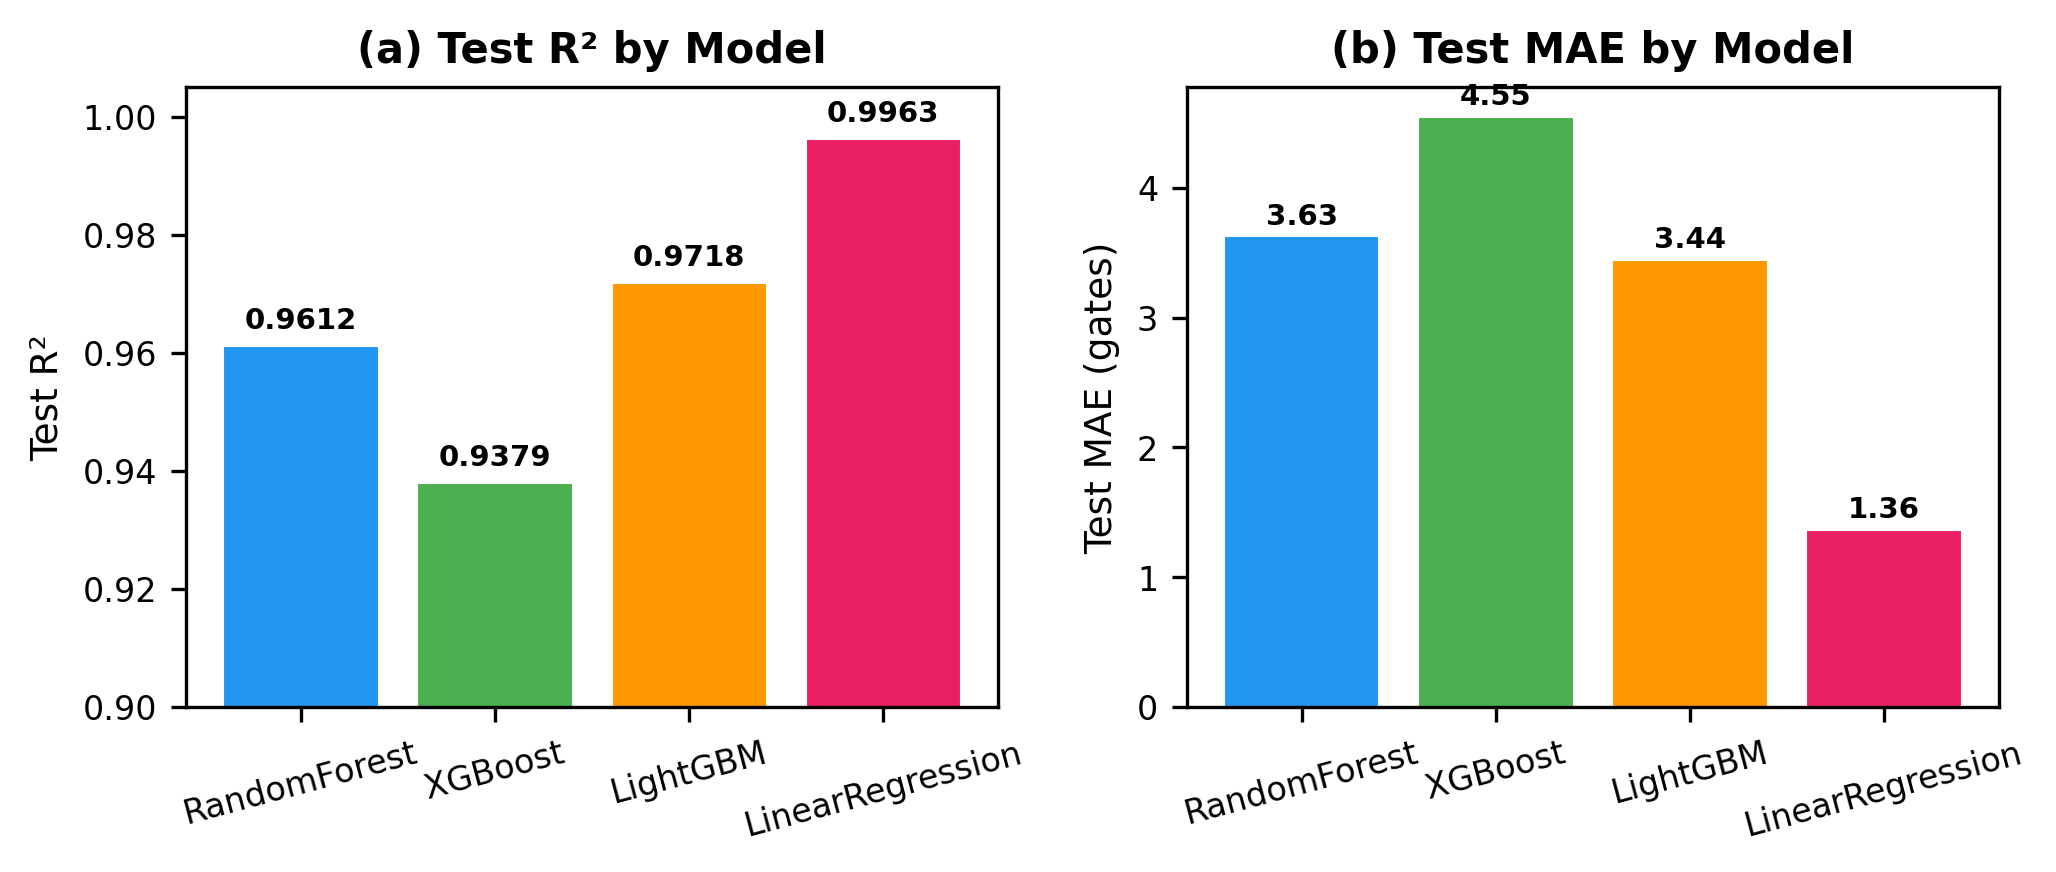
\includegraphics[width=\columnwidth]{model_comparison.png}
  \caption{Test $R^2$ and MAE across all four models. LinearRegression
  dominates both metrics, suggesting a near-linear feature--target
  relationship in the synthetic dataset.}
  \label{fig:model_comparison}
\end{figure}

\subsection{Cross-Validation and Learning Curve}

Five-fold cross-validation on the full 500-module dataset yields a mean
$R^2 = -0.124 \pm 0.097$ and mean MAE~$= 37.91 \pm 2.89$~gates. The
\textbf{negative mean $R^2$} is a genuine and reportable result: each fold
uses only 400 training samples (80\% of 500), and the high variance across
folds (per-fold $R^2$ ranging from $-0.317$ to $-0.068$) reflects the
limited dataset size rather than a fundamental model failure. The held-out
test set results (Table~\ref{tab:model_comparison}) use a fixed 350-sample
training set and show $R^2 > 0.93$ for all models, confirming that the CV
degradation is a sample-efficiency issue.

\begin{figure}[t]
  \centering
  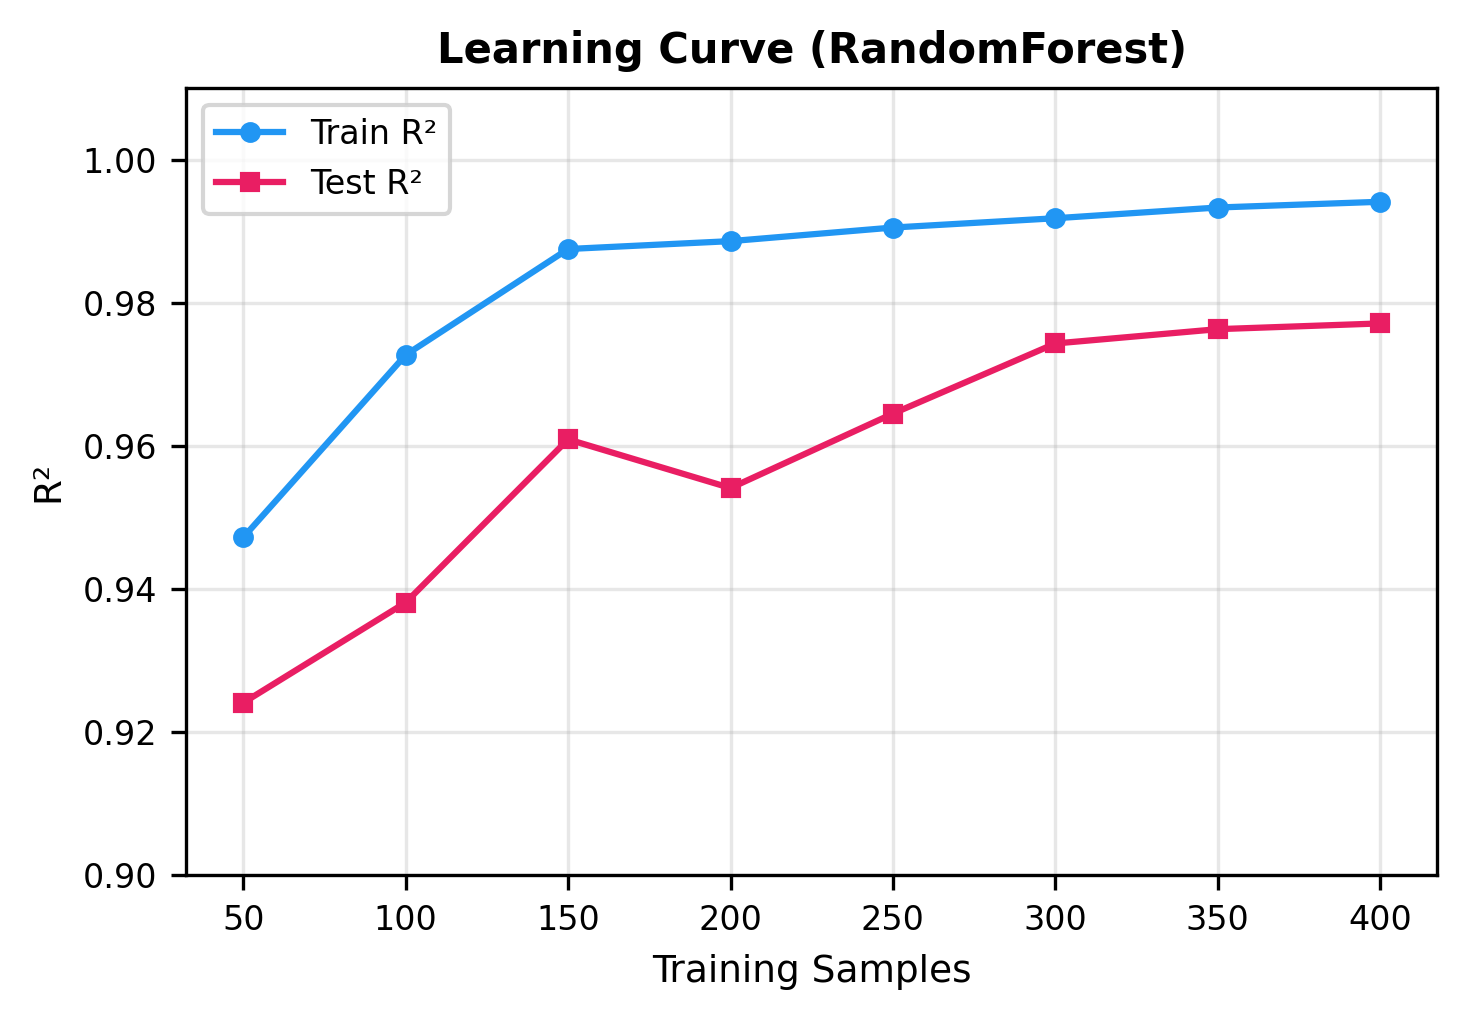
\includegraphics[width=\columnwidth]{learning_curve.png}
  \caption{Learning curve for RandomForest showing train and test $R^2$ as
  training set size increases from 50 to 400 samples. The persistent gap
  indicates potential for improvement with additional training data.}
  \label{fig:learning_curve}
\end{figure}

The learning curve (Fig.~\ref{fig:learning_curve}) shows monotonic
improvement in test $R^2$ from 0.9241 at $N{=}50$ to 0.9771 at $N{=}400$,
with a persistent train--test gap suggesting that additional data would
further reduce variance.

\subsection{Explainability and Faithfulness}

\begin{table}[t]
\centering
\caption{Faithfulness Verification: SHAP vs.\ Permutation Importance}
\label{tab:faithfulness}
\small
\begin{tabular}{@{}lcc@{}}
\toprule
\textbf{Metric} & \textbf{SHAP} & \textbf{Permutation} \\
\midrule
Faithfulness Score & 0.9768 & 0.9277 \\
Spearman $\rho$ & 0.9890 & 0.9396 \\
Spearman $p$-value & $1.75 \times 10^{-10}$ & $1.88 \times 10^{-6}$ \\
Kendall $\tau$ & 0.9487 & 0.8205 \\
Top-5 Overlap & 5/5 (100\%) & 4/5 (80\%) \\
Top-10 Overlap & 10/10 (100\%) & 10/10 (100\%) \\
\bottomrule
\end{tabular}
\end{table}

Table~\ref{tab:faithfulness} summarizes the faithfulness verification
results. SHAP achieves a higher faithfulness score (0.9768) with perfect
top-10 overlap and near-perfect rank correlation ($\rho = 0.989$). Permutation
Importance achieves 0.9277 with slightly lower rank correlation
($\rho = 0.940$) but still perfect top-10 overlap.

The primary disagreement occurs for \texttt{complex\_or\_gates}, which SHAP
ranks \#1 but ablation ranks \#5. This arises because OR gate counts are
highly collinear with \texttt{complex\_chars} and \texttt{complex\_nor\_gates}
in the training data. When \texttt{complex\_or\_gates} is ablated, the
Random Forest compensates by routing decisions through correlated features.
SHAP's coalitional tree-path allocation captures the marginal value without
retraining, while ablation permits full model adaptation. Conversely,
Permutation Importance over-ranks \texttt{complex\_chars} (\#1 vs.\ ablation
\#3) because independently shuffling character count creates unrealizable
feature combinations that push data points into out-of-distribution leaf
nodes, exaggerating the measured loss increase.

These disagreements are informative rather than problematic: they demonstrate
exactly why multi-method verification is necessary before deploying
XAI-informed decisions in production EDA workflows.

Table~\ref{tab:ranking} shows the top-5 feature ranking comparison across
all three methods, highlighting the specific rank shifts.

\begin{table}[t]
\centering
\caption{Top-5 Feature Ranking: Ablation vs.\ SHAP vs.\ Permutation}
\label{tab:ranking}
\footnotesize
\setlength{\tabcolsep}{2pt}
\begin{tabular}{@{}lccc@{}}
\toprule
\textbf{Feature} & \textbf{Ablation} & \textbf{SHAP} & \textbf{Perm.} \\
\midrule
complex\_nor\_gates  & \#1 (6.38)  & \#4 & \#3 \\
complex\_nand\_gates & \#2 (5.63)  & \#3 & \#4 \\
complex\_chars       & \#3 (5.09)  & \#5 & \textbf{\#1} \\
complex\_xor\_gates  & \#4 (5.01)  & \#2 & \#2 \\
complex\_or\_gates   & \#5 (3.17)  & \textbf{\#1} & \#6 \\
\bottomrule
\end{tabular}
\end{table}

\begin{figure}[t]
  \centering
  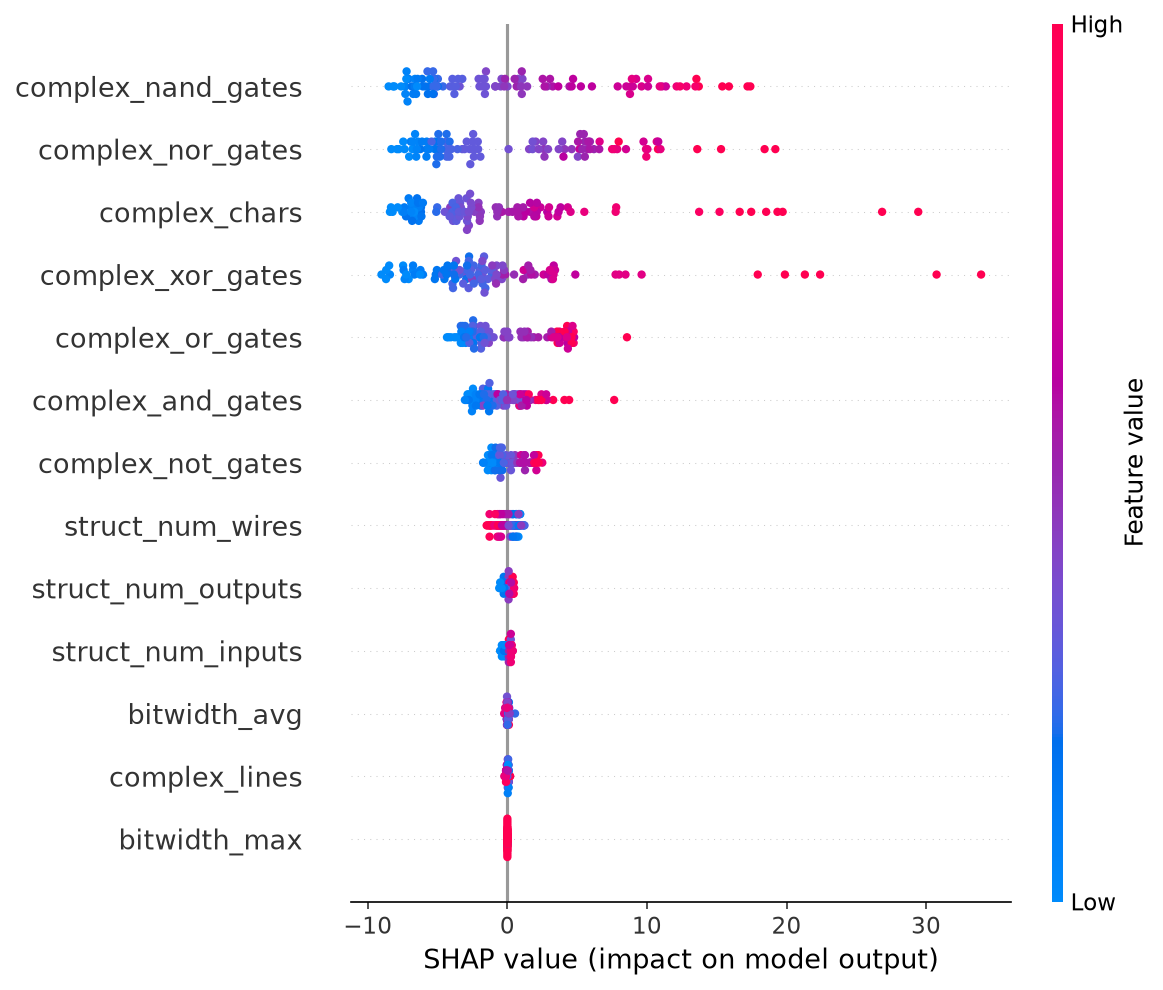
\includegraphics[width=\columnwidth]{shap_beeswarm.png}
  \caption{SHAP beeswarm plot showing feature contributions to predicted gate
  count across the test set.}
  \label{fig:shap}
\end{figure}

\subsection{Real-World Validation}

\begin{table}[t]
\centering
\caption{Real-World RTL Validation (All 17 Modules)}
\label{tab:real_world}
\footnotesize
\setlength{\tabcolsep}{3pt}
\begin{tabular}{@{}lrrrr@{}}
\toprule
\textbf{Module} & \textbf{Actual} & \textbf{Pred.} & \textbf{$|$Err$|$} & \textbf{Err\%} \\
\midrule
arbiter              & 15      & 44.76  & 29.76      & 198.4\% \\
axis\_adapter        & 18      & 45.31  & 27.31      & 151.7\% \\
axis\_arb\_mux       & 177     & 50.39  & 126.61     & 71.5\% \\
axis\_broadcast      & 60      & 45.29  & 14.71      & 24.5\% \\
axis\_crosspoint     & 228     & 45.27  & 182.73     & 80.2\% \\
axis\_demux          & 96      & 48.17  & 47.83      & 49.8\% \\
\textbf{axis\_fifo}  & \textbf{133{,}594} & \textbf{51.35} & \textbf{133{,}543} & \textbf{100.0\%} \\
axis\_mux            & 104     & 47.30  & 56.70      & 54.5\% \\
axis\_pipe.\_reg.    & 88      & 45.27  & 42.73      & 48.6\% \\
axis\_rate\_limit    & 462     & 47.67  & 414.33     & 89.7\% \\
axis\_register       & 44      & 45.31  & 1.31       & 3.0\% \\
i2c\_master          & 492     & 47.23  & 444.77     & 90.4\% \\
i2c\_master\_axil    & 4{,}092 & 47.20  & 4{,}044.80 & 98.9\% \\
priority\_encoder    & 7       & 43.59  & 36.59      & 522.7\% \\
uart                 & 420     & 43.54  & 376.46     & 89.6\% \\
uart\_rx             & 246     & 45.34  & 200.66     & 81.6\% \\
uart\_tx             & 171     & 43.15  & 127.85     & 74.8\% \\
\midrule
\multicolumn{5}{l}{\textit{All 17: $R^2 = -0.068$, MAE $= 8{,}218.69$ gates}} \\
\multicolumn{5}{l}{\textit{Excl.\ axis\_fifo (16): MAE $= 385.95$, Median $= 126.61$}} \\
\bottomrule
\end{tabular}
\end{table}


Table~\ref{tab:real_world} presents all 17 modules in the real-world
benchmark, sorted by module name. The overall $R^2 = -0.068$ and MAE~$= 8{,}218.69$~gates
are dominated by a single outlier: \texttt{axis\_fifo} synthesizes to
133{,}594 actual gates due to Yosys elaborating unmapped memory arrays
(\texttt{\$\_AND\_}, \texttt{\$\_OR\_}, etc.) without a technology library,
producing a gate count approximately three orders of magnitude larger than
any module in the training set.

Excluding \texttt{axis\_fifo}, the remaining 16 modules yield an MAE of
$385.95$~gates with a median absolute error of $126.61$~gates. While still
well above the in-distribution test MAE of $3.63$~gates, this confirms a
distributional shift rather than a fundamental model failure: the model's
predictions cluster around $43$--$51$~gates (the training distribution's
central tendency), demonstrating that feature extraction at the RTL level
captures structural patterns but lacks the dynamic range to extrapolate to
production-scale designs.

\begin{figure}[t]
  \centering
  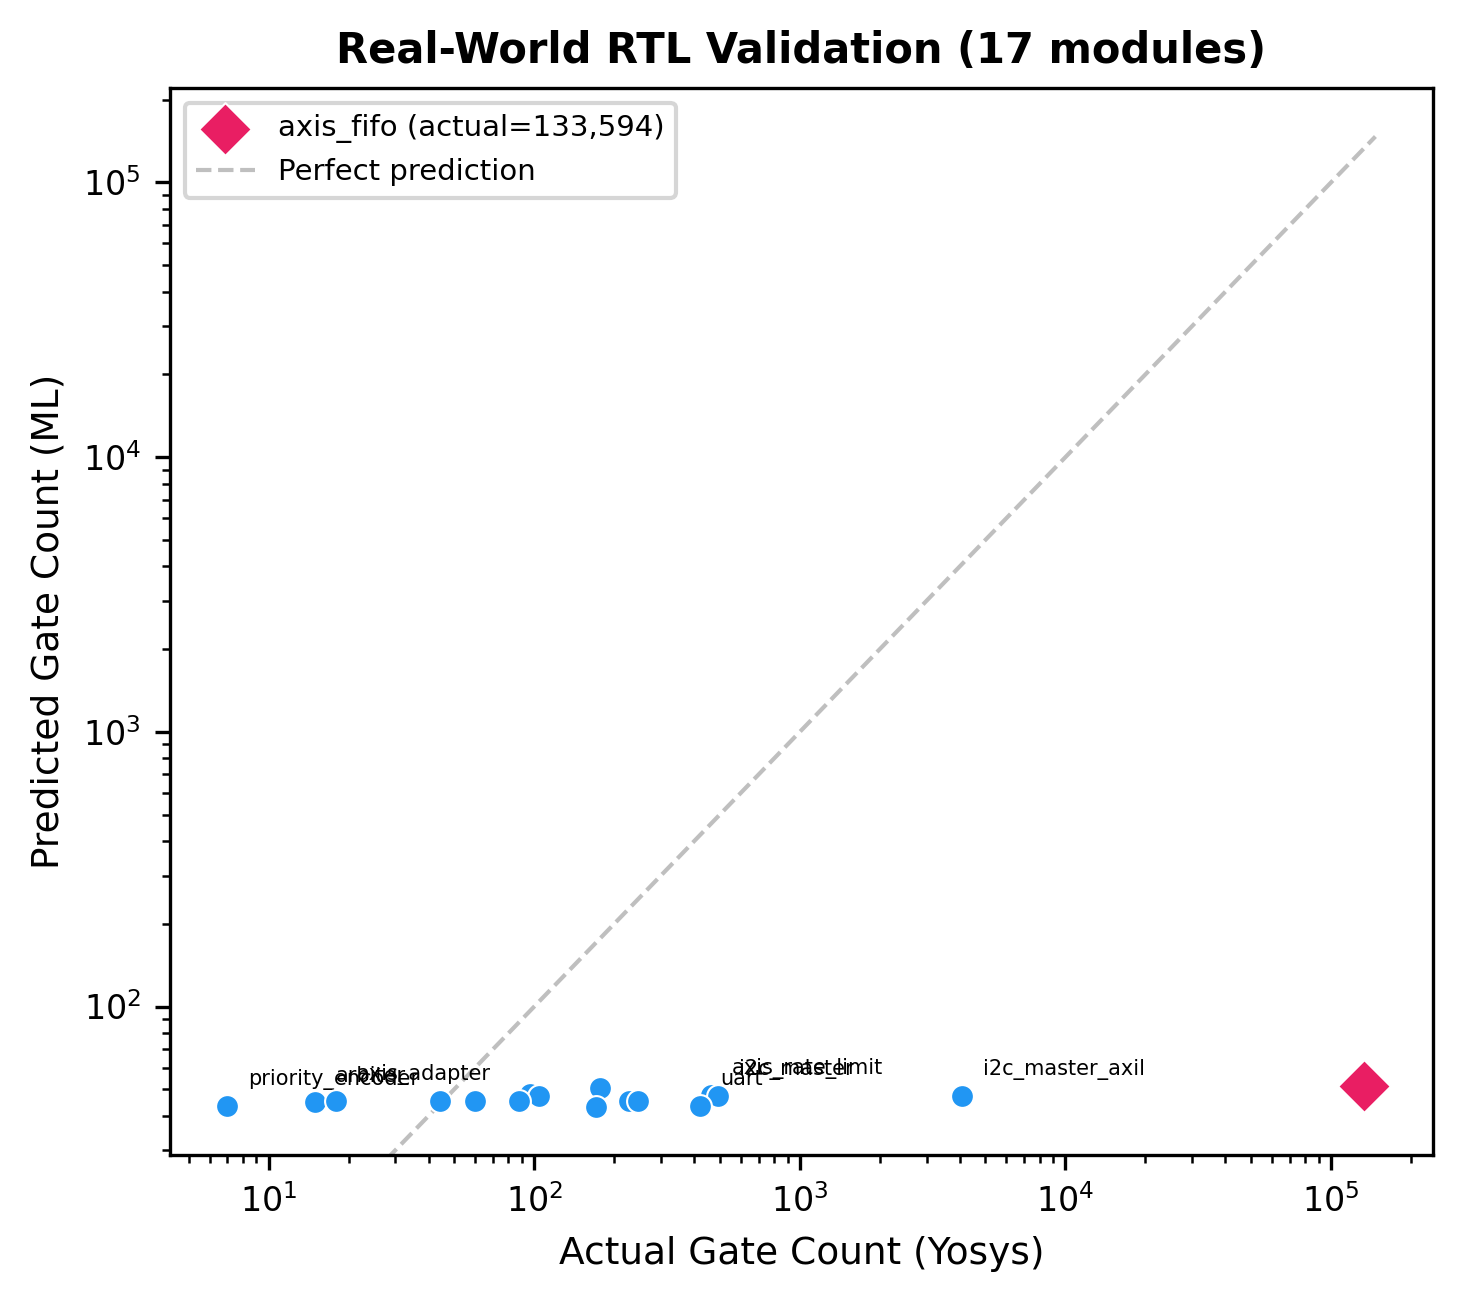
\includegraphics[width=\columnwidth]{real_world_scatter.png}
  \caption{Predicted vs.\ actual gate counts on 17 real-world modules
  (log-log scale). The \texttt{axis\_fifo} outlier (diamond) at
  133{,}594 actual gates is clearly marked.}
  \label{fig:scatter}
\end{figure}

\subsection{Inference Latency}

On 100 benchmark modules, ML batch inference requires $0.363$~ms per module
($36.33$~ms total), compared to $199.43$~ms per module ($19.94$~s total) for
real Yosys synthesis. This yields a verified speedup ratio of
$\mathbf{548.9\times}$ (99.82\% time saved).

% ============================================================================
% VI. DISCUSSION AND LIMITATIONS
% ============================================================================
\section{Discussion and Limitations}

\textbf{Dataset size.} The 500-module synthetic training set, while
sufficient for high in-distribution accuracy ($R^2 > 0.99$ for
LinearRegression), produces high cross-validation variance (mean CV
$R^2 = -0.124$). The learning curve suggests diminishing but non-zero
improvement at larger dataset sizes.

\textbf{Real-world generalization gap.} The out-of-distribution
$R^2 = -0.068$ on 17 real-world modules exposes a fundamental training
distribution mismatch. Predicted gate counts cluster narrowly
($43$--$51$~gates) while actual counts span five orders of magnitude
($7$--$133{,}594$~gates). This gap is exacerbated by the \texttt{axis\_fifo}
outlier, where Yosys elaborates unmapped memory constructs into primitive
logic gates without a technology library.

\textbf{Benchmark diversity.} The current real-RTL benchmark set contains
17~modules from a narrow domain (UART, I2C, AXI-Stream peripherals from
the \texttt{alexforencich} repositories) and does not yet cover structurally
diverse designs such as arithmetic-heavy ALUs, memory-dominated blocks, or
control-heavy finite state machines. Extending the benchmark to include
these categories is an immediate priority for future work.

\textbf{Linearity observation.} The dominance of LinearRegression on the
synthetic dataset is an important finding that should not be over-generalized.
It suggests that the hand-crafted features already encode gate-count
complexity linearly for the synthetic distribution; however, real-world
designs with more complex operator interactions, parameterized macros, and
memory instantiations are likely to require nonlinear models. Re-evaluating
all four models on a richer real-RTL training set is essential future work.

\textbf{Explainability verification generality.} Our ablation-based
faithfulness methodology is model-agnostic and can be applied to any
feature-attribution method. The disagreement analysis (Section~V-C) provides
a template for identifying multicollinearity-induced ranking artifacts that
would otherwise go undetected.

% ============================================================================
% VII. CONCLUSION
% ============================================================================
\section{Conclusion}

We presented AICD, a framework contributing three capabilities not jointly
present in prior RTL/EDA ML work: (1)~multi-model gate count prediction
achieving $R^2 = 0.9963$ with real Yosys synthesis ground truth;
(2)~dual-method explainability via SHAP and Permutation Importance; and
(3)~independent ablation-based faithfulness verification demonstrating
$\rho = 0.989$ rank correlation between SHAP attributions and empirical
model sensitivity.

The framework achieves a $548.9\times$ speedup over synthesis, with honest
reporting of the real-world generalization gap ($R^2 = -0.068$ on 17 real
modules). Future work will scale the training set, diversify the benchmark
suite, and investigate feature engineering for memory-heavy and
control-dominated designs.

% ============================================================================
% REFERENCES
% ============================================================================
\bibliographystyle{IEEEtran}
\bibliography{refs}

\end{document}
